\chapter{Electronic Spectra and Magnetism of Complexes}\label{ch:b3:complex-spectra-magnetism}

Ruby is red and emerald is green, yet both owe their colour to the same ion,
\ce{Cr^{3+}}, replacing a few aluminium ions in two different oxides: corundum,
$\ce{Al2O3}$, for the ruby, the beryllium aluminium silicate beryl for the emerald. In
both, the chromium sits in an octahedron of oxygen atoms; in beryl the
octahedron is a little larger and the ligand field a little weaker, and the
absorption bands of the ion move by about a thousand wavenumbers to the red.
That is enough to change the transmitted colour from red to green. This chapter
explains such spectra quantitatively: how the terms of a free ion split in a
ligand field, how \omterm{def:b3:complex-spectra-magnetism:tanabe-sugano}{Tanabe--Sugano diagrams} turn two band positions into the
ligand-field splitting and the electron repulsion, why some bands are intense
and others faint, why some complexes distort, and how magnetism counts the
unpaired electrons.

\begin{recall}
The Year 2 volume treated transition elements and their $d^n$ configurations,
crystal-field splitting $\Delta_{\mathrm o}$, high- and low-spin complexes, pairing energy,
crystal-field stabilisation energy, $d$--$d$ transitions, the spectrochemical
series, ligand field theory, and paramagnetic and diamagnetic substances.
\Cref{ch:b3:many-electron-atoms} derived \omterm{def:b3:many-electron-atoms:term}{term symbols} and Hund's rules,
\cref{ch:b3:group-theory-applied} reduced representations and \omterm{def:b3:group-theory-applied:direct-product}{direct products},
\cref{ch:b3:electronic-spectroscopy} stated the spin and Laporte selection rules
and described \omterm{def:b3:electronic-spectroscopy:charge-transfer}{charge-transfer transitions}, and
\cref{ch:b3:partition-functions} gave the \omterm{def:b3:partition-functions:boltzmann}{Boltzmann distribution}.
\end{recall}

\begin{omfigure}
\begin{minipage}[t]{0.3\linewidth}\centering
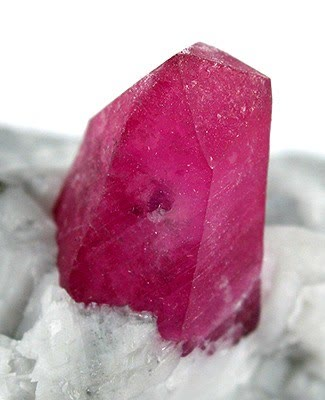
\includegraphics[height=4.2cm]{images/book4/ruby-crystal.jpg}\par
{\small ruby}
\end{minipage}\hspace{1.5em}
\begin{minipage}[t]{0.3\linewidth}\centering
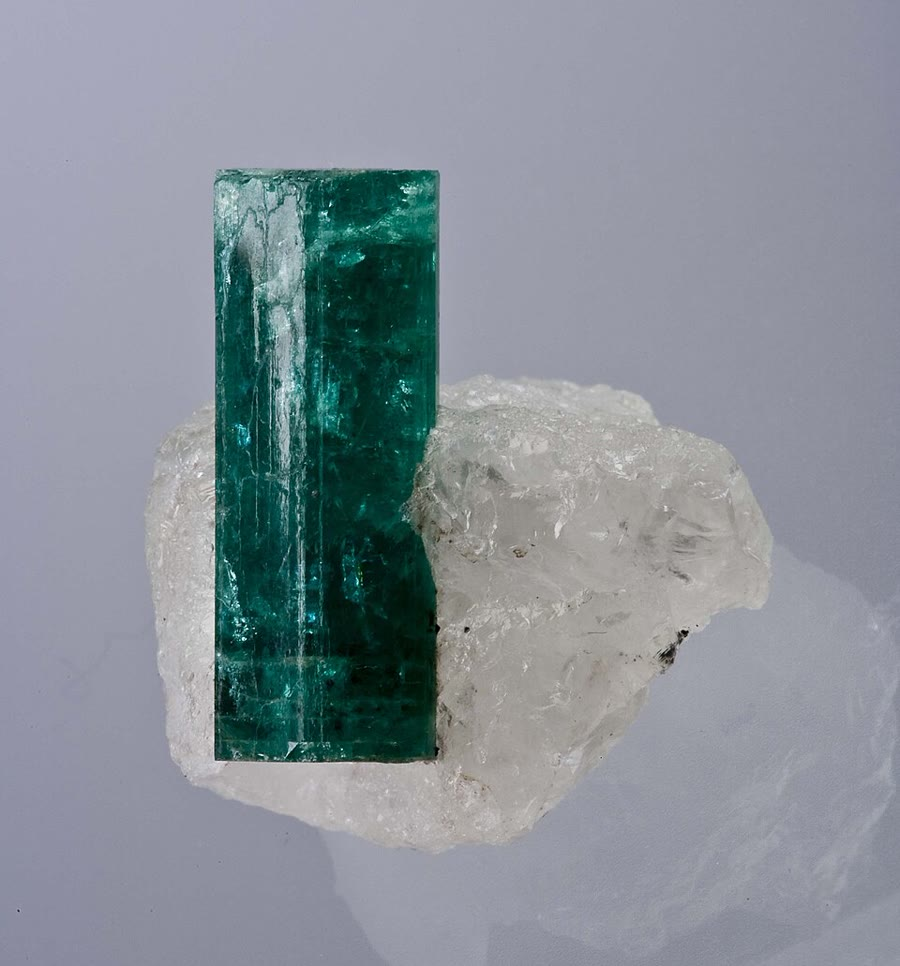
\includegraphics[height=4.2cm]{images/book4/emerald-crystal.jpg}\par
{\small emerald}
\end{minipage}

{\small A ruby crystal in marble and an emerald crystal on quartz. In both, the
colour comes from a few per cent of \ce{Cr^{3+}} in an octahedral site.}
\end{omfigure}

\section{From free-ion terms to ligand-field terms}

In a free ion the electron repulsion splits a $d^n$ configuration into terms
($^4$F, $^4$P, $^2$G\dots\ for $d^3$, \cref{ch:b3:many-electron-atoms}). In a complex, each term
is further split by the ligands, and the levels are labelled by the \omterm{def:b3:point-groups:irrep}{irreducible
representations} of the \omterm{def:b3:point-groups:point-group}{point group} of the complex.

\begin{definition}[Ligand-field term]\label{def:b3:complex-spectra-magnetism:ligand-field-term}
A \emph{ligand-field term}\index{ligand-field term} of a complex is a set of
degenerate many-electron states labelled by its \omterm{def:b3:many-electron-atoms:term}{spin multiplicity} and the
\omterm{def:b3:point-groups:irrep}{irreducible representation} of the \omterm{def:b3:point-groups:point-group}{point group} to which its orbital part
belongs, such as $^4$A$_{2g}$ or $^4$T$_{1g}$ in an octahedral complex.
\end{definition}

\begin{proposition}[Characters of the rotation group]\label{prop:b3:complex-spectra-magnetism:rotation-characters}
The $2L+1$ states of a term of orbital angular momentum $L$ form a representation
of the rotations whose \omterm{def:b3:point-groups:representation}{character} for a rotation by $\alpha$ is
\[
  \chi_L(\alpha) = \frac{\sin\bigl((L + \tfrac12)\alpha\bigr)}{\sin(\alpha/2)}, \qquad \chi_L(0) = 2L + 1 .
\]
\end{proposition}

\admitted

\begin{theorem}[Splitting of free-ion terms in an octahedral field]\label{thm:b3:complex-spectra-magnetism:term-splitting}
In an octahedral field the terms of a $d^n$ ion split into
\begin{center}
\begin{tabular}{ll}
\hline
free-ion term & octahedral terms (same \omterm{def:b3:many-electron-atoms:term}{spin multiplicity}) \\ \hline
S & A$_{1g}$ \\
P & T$_{1g}$ \\
D & E$_g$ + T$_{2g}$ \\
F & A$_{2g}$ + T$_{1g}$ + T$_{2g}$ \\
G & A$_{1g}$ + E$_g$ + T$_{1g}$ + T$_{2g}$ \\ \hline
\end{tabular}
\end{center}
\end{theorem}

\begin{proof}
The octahedral group is the rotation group $O$ times the inversion; the $d$ functions
are even, so every term of a $d^n$ configuration is even ($g$), and it is enough to
reduce in $O$, whose classes are $E$, $8C_3$, $3C_2$ ($=C_4^2$), $6C_4$ and $6C_2'$. With the
proposition, for $L = 3$: $\chi = 7$, $\sin(420^\circ)/\sin60^\circ = 1$, $\sin(630^\circ)/\sin90^\circ = -1$, $\sin(315^\circ)/\sin45^\circ = -1$
and $-1$. The \omterm{def:b3:point-groups:irrep}{character table} of $O$ (rows $A_1$: 1, 1, 1, 1, 1; $A_2$: 1, 1, 1, $-1$, $-1$; $E$: 2,
$-1$, 2, 0, 0; $T_1$: 3, 0, $-1$, 1, $-1$; $T_2$: 3, 0, $-1$, $-1$, 1) and the \omterm{thm:b3:group-theory-applied:reduction}{reduction formula} of
\cref{ch:b3:group-theory-applied} give $n(A_2) = (7 + 8 - 3 + 6 + 6)/24 = 1$, $n(T_1) = (21 + 3 - 6 +
6)/24 = 1$, $n(T_2) = (21 + 3 + 6 - 6)/24 = 1$, and zero for $A_1$ and $E$. The other rows are
obtained in the same way ($L = 0$: $(1, 1, 1, 1, 1)$; $L = 1$: $(3, 0, -1, 1, -1)$; $L = 2$: $(5, -1, 1,
-1, 1)$; $L = 4$: $(9, 0, 1, 1, 1)$).
\end{proof}

\begin{method}[Splitting a free-ion term]\label{met:b3:complex-spectra-magnetism:split-term}
\begin{enumerate}
  \item Find the ground term of the free ion (Hund's rules) and the excited
        terms of the same multiplicity.
  \item Read their octahedral components in the table; the \omterm{def:b3:many-electron-atoms:term}{spin multiplicity} is
        unchanged.
  \item Order them: for the ground F term of $d^2$, $d^7$ (high spin) the lowest is T$_{1g}$;
        for $d^3$, $d^8$ it is A$_{2g}$ (next proposition).
\end{enumerate}
\end{method}

\begin{proposition}[Holes and the tetrahedral inversion]\label{prop:b3:complex-spectra-magnetism:hole}
The terms of $d^{10-n}$ in an octahedral field are those of $d^n$ in reverse energy
order; the terms of $d^n$ in a tetrahedral field are those of $d^{10-n}$ in an octahedral
field (with the $g$ subscripts dropped).
\end{proposition}

\begin{proof}
A $d^{10-n}$ configuration is equivalent to $n$ positive holes in a full shell: the
holes feel the ligand-field potential with the opposite sign, so every
one-electron splitting, and hence every term splitting, is reversed (the
electron repulsion between holes is the same as between electrons). A
tetrahedral field has the opposite sign of an octahedral one (the $e$ orbitals
lie lower) and no centre of symmetry: $d^n$ in $T_d$ behaves as $d^n$ with a reversed
field, i.e. as $d^{10-n}$ in $O_h$.
\end{proof}

\begin{definition}[Correlation diagram]\label{def:b3:complex-spectra-magnetism:correlation}
A \emph{correlation diagram}\index{correlation diagram} joins the states of a
system in two limiting situations, here the free-ion terms split by a weak
field and the configurations $t_{2g}^ae_g^b$ of a strong field, connecting states of the
same symmetry without letting two of them cross.
\end{definition}

\begin{omfigure}
\begin{tikzpicture}[font=\small]
  % free ion
  \pic (F) at (0,0) {omlevel={}{1.1}};
  \pic (P) at (0,3.0) {omlevel={}{1.1}};
  \node[anchor=east] at (F-l) {$^3$F};
  \node[anchor=east] at (P-l) {$^3$P};
  % weak field
  \pic (a) at (2.6,-0.8) {omlevel={}{1.0}};
  \pic (b) at (2.6,0.3) {omlevel={}{1.0}};
  \pic (c) at (2.6,1.4) {omlevel={}{1.0}};
  \pic (d) at (2.6,3.1) {omlevel={}{1.0}};
  \foreach \n/\t in {a/T$_{1g}$, b/T$_{2g}$, c/A$_{2g}$, d/T$_{1g}$(P)}{\node[omsymlabel, anchor=south] at (\n-c) {$^3$\t};}
  \draw[omcorr] (F-r) -- (a-l) (F-r) -- (b-l) (F-r) -- (c-l) (P-r) -- (d-l);
  % strong field configurations
  \pic (A) at (7.4,-1.6) {omlevel={}{1.0}};
  \pic (B) at (7.4,1.4) {omlevel={}{1.0}};
  \pic (C) at (7.4,1.9) {omlevel={}{1.0}};
  \pic (D) at (7.4,4.6) {omlevel={}{1.0}};
  \node[anchor=west] at (A-r) {$^3$T$_{1g}$ \quad $t_{2g}^2$};
  \node[anchor=west] at (B-r) {$^3$T$_{2g}$};
  \node[anchor=west] at (C-r) {$^3$T$_{1g}$ \quad $t_{2g}e_g$};
  \node[anchor=west] at (D-r) {$^3$A$_{2g}$ \quad $e_g^2$};
  \draw[omcorr] (a-r) -- (A-l) (b-r) -- (B-l) (c-r) -- (D-l) (d-r) -- (C-l);
  \node[anchor=north] at (0,-2.0) {free ion};
  \node[anchor=north] at (2.6,-2.0) {weak field};
  \node[anchor=north] at (7.4,-2.0) {strong field};
  \draw[->, black!50] (3.7,-2.3) -- (6.2,-2.3) node[midway, below, font=\scriptsize] {increasing $\Delta_{\mathrm o}$};
\end{tikzpicture}

{\small \omterm{def:b3:complex-spectra-magnetism:correlation}{Correlation diagram} of the \omterm{def:b3:many-electron-atoms:singlet-triplet}{triplet states} of a $d^2$ ion in an octahedral
field. Each weak-field term goes to the strong-field configuration of the same
symmetry, and the two $^3$T$_{1g}$ states do not cross: the lower goes to $t_{2g}^2$, the upper to
$t_{2g}e_g$.}
\end{omfigure}

\section{Tanabe--Sugano diagrams}

\begin{definition}[Racah parameters]\label{def:b3:complex-spectra-magnetism:racah}
The \emph{Racah parameters}\index{Racah parameters} $A$, $B$ and $C$ are combinations of
the Slater integrals of the $d$ shell that express all the electron-repulsion
energies of a $d^n$ configuration; the energy differences between terms of the
same configuration depend only on $B$ and $C$, and those between terms of the same
highest multiplicity on $B$ alone (for $d^2$, $d^3$, $d^7$, $d^8$: $E(\mathrm P) - E(\mathrm F) = 15B$).
\end{definition}

\begin{example}[Free-ion Racah parameters]\label{ex:b3:complex-spectra-magnetism:free-B}
% ledger: lev:Cr3.4F5_2, lev:Cr3.4F7_2, lev:Cr3.4F9_2, lev:Cr3.4P1_2, lev:Cr3.4P3_2, lev:Cr3.4P5_2, lev:Ni2.3F3, lev:Ni2.3F2, lev:Ni2.3P2, lev:Ni2.3P1, lev:Ni2.3P0, lev:V2.4F5_2, lev:V2.4F7_2, lev:V2.4F9_2, lev:V2.4P1_2, lev:V2.4P3_2, lev:V2.4P5_2
The levels of the free \ce{Cr^{3+}} ion put the centre of gravity (weights $2J + 1$) of $^4$F at
\qty{547}{cm^{-1}} and that of $^4$P at \qty{14305}{cm^{-1}} above the ground level: $15B = \qty{13758}{cm^{-1}}$,
$B = \qty{917}{cm^{-1}}$. The same calculation gives $B = 755$ for \ce{V^{2+}} and \qty{1056}{cm^{-1}} for
\ce{Ni^{2+}}.
\end{example}

\begin{definition}[Tanabe--Sugano diagram]\label{def:b3:complex-spectra-magnetism:tanabe-sugano}
A \emph{Tanabe--Sugano diagram}\index{Tanabe--Sugano diagram} plots the energies of
all the \omterm{def:b3:complex-spectra-magnetism:ligand-field-term}{ligand-field terms} of a $d^n$ ion, in units of $B$ and measured from the
ground term, against $\Delta_{\mathrm o}/B$, for a fixed ratio $C/B$.
\end{definition}

\begin{proposition}[The three bands of a $d^3$ ion]\label{prop:b3:complex-spectra-magnetism:d3-bands}
For a $d^3$ ion in an octahedral field the spin-allowed transitions from $^4$A$_{2g}$ are at
\[
  \nu_1 = \Delta_{\mathrm o}\ (^4\mathrm T_{2g}), \qquad
  \nu_{2,3} = 7.5B + 1.5\Delta_{\mathrm o} \mp \tfrac12\sqrt{225B^2 - 18B\Delta_{\mathrm o} + \Delta_{\mathrm o}^2}\ (^4\mathrm T_{1g}(\mathrm F), {}^4\mathrm T_{1g}(\mathrm P)).
\]
\end{proposition}

\begin{proof}[Partial proof]
In the strong-field basis, $^4$A$_{2g}$ and $^4$T$_{2g}$ arise once each, from $t_{2g}^3$ and $t_{2g}^2e_g$, and
their difference contains no electron repulsion: $\nu_1 = \Delta_{\mathrm o}$ exactly. $^4$T$_{1g}$ arises
twice, from $t_{2g}^2e_g$ and $t_{2g}e_g^2$; relative to $^4$A$_{2g}$ the $2\times2$ matrix is
$\begin{pmatrix}\Delta_{\mathrm o} + 12B & 6B\\ 6B & 2\Delta_{\mathrm o} + 3B\end{pmatrix}$ (the electron-repulsion elements are admitted).
Its \omterm{def:b3:quantum-model-systems:operator}{eigenvalues} are the roots of $E^2 - (15B + 3\Delta_{\mathrm o})E + 2\Delta_{\mathrm o}^2 + 27B\Delta_{\mathrm o} = 0$, which are the stated
$\nu_2$ and $\nu_3$. At $\Delta_{\mathrm o} = 0$ they are 0 and $15B$ (the $^4$F and $^4$P terms); the full
diagonalisation of the figure reproduces them.
\end{proof}

\begin{omfigure}
\begin{tikzpicture}
\begin{axis}[name=ta, omts, width=0.46\linewidth, height=7.0cm, xmin=1, xmax=40, ymin=0, ymax=70,
  xlabel={$\Delta_{\mathrm o}/B$}, ylabel={$E/B$}, title={\small $d^3$, $C/B = 4.5$},
  unbounded coords=jump, clip=true, clip mode=individual]
\foreach \c in {f0,f1,f2,f3,f4,f5,f6,f7,f8,f9,f10,f11,f12,f13,f14,f15}{
  \addplot[omtsforbidden, restrict x to domain=1:40] table[x=x, y=\c] {figdata/out/bachelor-3-tanabe-sugano-d3.dat};}
\foreach \c in {a0,a1,a2,a3}{
  \addplot[omDef, thick, restrict x to domain=1:40] table[x=x, y=\c] {figdata/out/bachelor-3-tanabe-sugano-d3.dat};}
\draw[omThm, dashed] (axis cs:29.0,0) -- (axis cs:29.0,70);
\draw[black!70, dashed] (axis cs:27.1,0) -- (axis cs:27.1,70);
\node[font=\scriptsize, omThm, anchor=north west, rotate=90] at (axis cs:29.6,1.5) {ruby};
\node[font=\scriptsize, anchor=south west, rotate=90] at (axis cs:26.6,1.5) {emerald};
% labels outside the frame, at the height where each curve leaves it
\node[font=\scriptsize, omDef, anchor=west, inner sep=1pt] at (axis cs:40,40) {$^4$T$_{2g}$};
\node[font=\scriptsize, omDef, anchor=west, inner sep=1pt] at (axis cs:40,50.9) {$^4$T$_{1g}$};
\node[font=\scriptsize, omDef, anchor=south, inner sep=1pt] at (axis cs:32.8,70) {$^4$T$_{1g}$(P)};
\node[font=\scriptsize, black!60, anchor=west, inner sep=1pt] at (axis cs:40,21.2) {$^2$E$_g$};
\end{axis}
\begin{axis}[at={(ta.east)}, anchor=west, xshift=2.2cm, omts, width=0.46\linewidth, height=7.0cm,
  xmin=1, xmax=40, ymin=0, ymax=70, xlabel={$\Delta_{\mathrm o}/B$}, ylabel={$E/B$},
  title={\small $d^8$, $C/B = 4.71$}, unbounded coords=jump, clip=true, clip mode=individual]
\foreach \c in {f0,f1,f2,f3,f4,f5,f6}{
  \addplot[omtsforbidden, restrict x to domain=1:40] table[x=x, y=\c] {figdata/out/bachelor-3-tanabe-sugano-d8.dat};}
\foreach \c in {a0,a1,a2,a3}{
  \addplot[omDef, thick, restrict x to domain=1:40] table[x=x, y=\c] {figdata/out/bachelor-3-tanabe-sugano-d8.dat};}
\node[font=\scriptsize, omDef, anchor=west, inner sep=1pt] at (axis cs:40,40) {$^3$T$_{2g}$};
\node[font=\scriptsize, omDef, anchor=west, inner sep=1pt] at (axis cs:40,50.9) {$^3$T$_{1g}$};
\node[font=\scriptsize, omDef, anchor=south, inner sep=1pt] at (axis cs:32.8,70) {$^3$T$_{1g}$(P)};
\end{axis}
\end{tikzpicture}

{\small \omterm{def:b3:complex-spectra-magnetism:tanabe-sugano}{Tanabe--Sugano diagrams} of $d^3$ and $d^8$ ions computed by diagonalising the
ligand-field and electron-repulsion Hamiltonian over all the states of the
configuration. Thick blue: the states of the ground-state multiplicity
(spin-allowed transitions); thin grey: the others. The ground term is the
horizontal axis ($^4$A$_{2g}$ for $d^3$, $^3$A$_{2g}$ for $d^8$). Dashed: ruby and emerald, placed at the $\Delta_{\mathrm o}/B$ of their two bands.
The $^2$E$_g$ level of $d^3$ is almost flat: its energy hardly depends on the field.}
\end{omfigure}

\begin{method}[Reading a Tanabe--Sugano diagram]\label{met:b3:complex-spectra-magnetism:read-ts}
\begin{enumerate}
  \item Identify the ground term and the spin-allowed transitions (same
        multiplicity).
  \item Compute the ratio of two band energies, $\nu_2/\nu_1$; find the value of $\Delta_{\mathrm o}/B$ at
        which the diagram gives that ratio.
  \item Read $E/B$ for $\nu_1$ there: $B = \nu_1/(E/B)$, then $\Delta_{\mathrm o}$. For $d^3$ and $d^8$, $\Delta_{\mathrm o} = \nu_1$
        directly and the closed formula gives $B$ from $\nu_2$.
  \item Compare $B$ with the free-ion value (\omterm{def:b3:complex-spectra-magnetism:nephelauxetic}{nephelauxetic ratio}) and check that the
        third band falls where the diagram predicts.
\end{enumerate}
\end{method}

\begin{definition}[Nephelauxetic effect]\label{def:b3:complex-spectra-magnetism:nephelauxetic}
The \emph{nephelauxetic effect}\index{nephelauxetic effect} (``cloud-expanding'') is
the decrease of the Racah parameter $B$ of a metal ion in a complex compared with
the free ion, caused by the delocalisation of the $d$ electrons onto the
ligands; the \emph{nephelauxetic ratio}\index{nephelauxetic ratio} is $\beta =
B_{\text{complex}}/B_{\text{free ion}}$.
\end{definition}

Ligands that bond more covalently reduce $B$ more: $\beta$ is near 0.9 for fluoride, 0.8
for water, 0.6 to 0.7 for oxide and heavier halides, and lower still for sulfide.
Spin-forbidden transitions, between terms of different multiplicity, appear
as weak, often sharp lines.

\section{Intensities and charge transfer}

\begin{definition}[Vibronic coupling]\label{def:b3:complex-spectra-magnetism:vibronic-coupling}
\emph{Vibronic coupling}\index{vibronic coupling} is the mixing of electronic and
vibrational motion: an asymmetric vibration that removes the centre of
symmetry of a complex mixes a little odd ($u$) character into its $d$ states,
which makes Laporte-forbidden $d$--$d$ transitions weakly allowed.
\end{definition}

\begin{proposition}[Intensities of absorption bands]\label{prop:b3:complex-spectra-magnetism:intensity-order}
The molar absorption coefficients of the bands of complexes increase in the
order: spin-forbidden $d$--$d$ $\ll$ spin-allowed $d$--$d$ in a centrosymmetric complex $<$ $d$--$d$
in a tetrahedral complex $<$ charge transfer.
\end{proposition}

\begin{proof}[Argued]
By \cref{ch:b3:electronic-spectroscopy}, a transition is allowed when spin is
conserved and parity changes. A $d$--$d$ transition never changes parity: in an
octahedral complex it borrows intensity only through \omterm{def:b3:complex-spectra-magnetism:vibronic-coupling}{vibronic coupling}; in a
tetrahedron, which has no centre, $d$ and $p$ orbitals mix permanently. A
spin-forbidden transition borrows a further small fraction through \omterm{def:b3:many-electron-atoms:spin-orbit}{spin--orbit
coupling}. A \omterm{def:b3:electronic-spectroscopy:charge-transfer}{charge-transfer transition} moves an electron between orbitals of
different parity on metal and ligand, and is fully allowed.
\end{proof}

\begin{definition}[Charge transfer]\label{def:b3:complex-spectra-magnetism:ct}
In a \emph{ligand-to-metal charge transfer}\index{ligand-to-metal charge
transfer} (LMCT) an electron goes from a ligand-based orbital to a metal-based
one; in a \emph{metal-to-ligand charge transfer}\index{metal-to-ligand charge
transfer} (MLCT), from the metal to a ligand $\pi^*$ orbital.
\end{definition}

Permanganate and chromate, $d^0$ ions with no $d$--$d$ transitions at all, owe their deep
colours to LMCT from oxide to an empty metal $d$ orbital, easy for a metal in a high
oxidation state. $\ce{[Ru(bpy)3]^{2+}}$ (bpy: 2,2$'$-bipyridine) owes its orange colour to MLCT
from ruthenium(II) to the $\pi^*$ orbitals of the ligands, the excited state used in
\omterm{def:b3:photochemistry:photoredox}{photoredox catalysis} (\cref{ch:b3:photochemistry}). In ruby, the two broad bands
near 560 and \qty{410}{nm} are the spin-allowed $d$--$d$ bands of
\cref{prop:b3:complex-spectra-magnetism:d3-bands}; the light that passes is red,
with some blue. Excited into these bands, the ion relaxes to the $^2$E$_g$ level and
emits from it the deep red R line near \qty{695}{nm}, the line of the first laser.

\section{The Jahn--Teller effect}

\begin{theorem}[Jahn--Teller theorem]\label{thm:b3:complex-spectra-magnetism:jahn-teller}
A non-linear molecule in an orbitally degenerate electronic state is unstable
with respect to a distortion that lowers its symmetry and removes the
\omterm{def:b3:quantum-model-systems:degenerate}{degeneracy}. This is the \emph{Jahn--Teller theorem}\index{Jahn--Teller theorem}.
\end{theorem}

\admitted

Its consequences for octahedral complexes follow from the occupation of the
$e_g$ orbitals, which point at the ligands. In a $d^9$ ion (\ce{Cu^{2+}}) the configuration
$t_{2g}^6e_g^3$ has the hole either in $d_{z^2}$ or in $d_{x^2-y^2}$: an E$_g$ state. Stretching the two axial
bonds lowers $d_{z^2}$ and raises $d_{x^2-y^2}$; putting two electrons in the lowered orbital
and one in the raised one gives a net stabilisation. Copper(II) complexes are
indeed elongated octahedra, with four short and two long bonds. The same holds
for high-spin $d^4$ (\ce{Mn^{3+}}, \ce{Cr^{2+}}) and low-spin $d^7$; for unevenly filled $t_{2g}$ sets
($d^1$, $d^2$, low-spin $d^5$\dots) the orbitals point between the ligands and the
distortion is small. The degenerate excited states of complexes distort too: the
broad, often double-humped bands of \ce{[Ti(H2O)6]^{3+}} and of copper(II) complexes are
the spectroscopic signature.

\begin{omfigure}
\begin{tikzpicture}[font=\small]
  \pic[transform shape] (t) at (0,0) {omlevel={}{1.6}};
  \pic[transform shape] (e) at (0,2.2) {omlevel={}{1.1}};
  \node[anchor=east] at (t-l) {$t_{2g}$};
  \node[anchor=east] at (e-l) {$e_g$};
  \pic[transform shape] (xy) at (4.2,0.45) {omlevel={ud}{0.8}};
  \pic[transform shape] (xz) at (4.2,-0.25) {omlevel={ud}{1.4}};
  \pic[transform shape] (x2) at (4.2,3.0) {omlevel={u}{0.8}};
  \pic[transform shape] (z2) at (4.2,1.5) {omlevel={ud}{0.8}};
  \draw[omcorr] (t-r) -- (xy-l) (t-r) -- (xz-l) (e-r) -- (x2-l) (e-r) -- (z2-l);
  \node[anchor=west] at (xy-r) {$b_{2g}$ ($d_{xy}$)};
  \node[anchor=west] at (xz-r) {$e_g$ ($d_{xz}$, $d_{yz}$)};
  \node[anchor=west] at (x2-r) {$b_{1g}$ ($d_{x^2-y^2}$)};
  \node[anchor=west] at (z2-r) {$a_{1g}$ ($d_{z^2}$)};
  \node[anchor=north] at (0,-0.9) {$O_h$};
  \node[anchor=north] at (4.2,-0.9) {$D_{4h}$, elongated};
  \begin{scope}[xshift=9.0cm, yshift=1.2cm, scale=0.8]
    \pic[transform shape] {omoctahedron};
    \draw[->, thick, omThm] (0,1.25) -- (0,1.85);
    \draw[->, thick, omThm] (0,-1.25) -- (0,-1.85);
  \end{scope}
\end{tikzpicture}

{\small Jahn--Teller distortion of a $d^9$ octahedral complex: stretching the axial bonds (right) splits $e_g$ into $a_{1g}$
($d_{z^2}$, lowered) and $b_{1g}$ ($d_{x^2-y^2}$, raised), and $t_{2g}$ into $e_g$ and $b_{2g}$. With nine
electrons the single hole sits in $b_{1g}$: the distortion is a net stabilisation.}
\end{omfigure}

\section{Magnetism}

\begin{definition}[Magnetic susceptibility]\label{def:b3:complex-spectra-magnetism:susceptibility}
The \emph{magnetic susceptibility}\index{magnetic susceptibility} $\chi$ of a material
is the ratio of its magnetisation to the applied field strength; the \emph{molar
susceptibility}\index{molar susceptibility} $\chi_{\mathrm m}$ is the susceptibility per mole.
Paramagnetic substances have $\chi > 0$, diamagnetic ones a small $\chi < 0$. Chemists often
use the cgs value of $\chi_{\mathrm m}$, in \unit{cm^3.mol^{-1}}, equal to the SI value in \unit{m^3.mol^{-1}}
divided by $4\pi\times10^{-6}$.
\end{definition}

\begin{definition}[Curie constant]\label{def:b3:complex-spectra-magnetism:curie}
The \emph{Curie constant}\index{Curie constant} $C$ of a paramagnet obeying the
\omterm{thm:b3:complex-spectra-magnetism:curie}{Curie law} is the product $\chi_{\mathrm m}T$.
\end{definition}

\begin{theorem}[Curie law]\label{thm:b3:complex-spectra-magnetism:curie}
For independent spins $S$ with $g$ factor $g$, at temperatures where $g\mu_BB \ll kT$,
\[
  \chi_{\mathrm m} = \frac{C}{T}, \qquad C = \frac{\mu_0N_Ag^2\mu_B^2S(S+1)}{3k}\ \ (\text{SI});
\]
in cgs units $C = 0.1251\,g^2S(S+1)$ \unit{cm^3.K.mol^{-1}}. This is the \emph{Curie law}\index{Curie law}.
\end{theorem}

\begin{proof}[Partial proof]
For $S = \frac12$, the two levels $m_S = \pm\frac12$ have energies $\pm\frac12g\mu_BB$ in a field $B$. By the
\omterm{def:b3:partition-functions:boltzmann}{Boltzmann distribution} the mean moment along the field is $\frac12g\mu_B\tanh(g\mu_BB/2kT) \approx
g^2\mu_B^2B/4kT$; per mole, $M = N_Ag^2\mu_B^2B/4kT$, and with $\chi_{\mathrm m} = \mu_0M/B$, $\chi_{\mathrm m} = \mu_0N_Ag^2\mu_B^2/(4kT)$,
which is the formula with $S(S+1) = \frac34$. The general case (averaging $m_S^2$ over $2S + 1$
levels, $\langle m_S^2\rangle = S(S+1)/3$) is admitted.
\end{proof}

\begin{definition}[Effective magnetic moment]\label{def:b3:complex-spectra-magnetism:moment}
The \emph{effective magnetic moment}\index{effective magnetic moment} of a
paramagnetic ion is $\mu_{\mathrm{eff}} = \sqrt{3k\chi_{\mathrm m}T/(\mu_0N_A)}$, in cgs $\mu_{\mathrm{eff}}/\mu_B = 2.828\sqrt{\chi_{\mathrm m}T}$. Its
\emph{spin-only moment}\index{spin-only moment} is the value $2\sqrt{S(S+1)}\,\mu_B$ that the
spins alone would give with $g = 2$; the excess of the measured moment over it is
the \emph{orbital contribution}\index{orbital contribution}.
\end{definition}

\begin{proposition}[Spin-only formula]\label{prop:b3:complex-spectra-magnetism:spin-only}
For $n$ unpaired electrons, $\mu_{\text{spin only}} = \sqrt{n(n+2)}\,\mu_B$: 1.73, 2.83, 3.87, 4.90 and $5.92\,\mu_B$ for
$n = 1$ to 5.
\end{proposition}

\begin{proof}
$S = n/2$, so $2\sqrt{S(S+1)} = 2\sqrt{\frac n2(\frac n2 + 1)} = \sqrt{n(n+2)}$.
\end{proof}

\begin{proposition}[Orbital contributions]\label{prop:b3:complex-spectra-magnetism:orbital-contribution}
In an octahedral complex, ions with A or E ground terms have moments close to the
spin-only value; ions with T ground terms can have substantial \omterm{def:b3:complex-spectra-magnetism:moment}{orbital
contributions}.
\end{proposition}

\begin{proof}[Argued]
An orbital moment needs an orbital that can be turned into an equivalent,
degenerate one by a rotation about the field axis, with an electron free to
move between them. In a T state ($t_{2g}$ set unevenly filled) the orbitals $d_{xz}$, $d_{yz}$, $d_{xy}$
are related by $90^\circ$ rotations and the moment survives in part; in A and E states
($t_{2g}^3$, $t_{2g}^6e_g^2$, $e_g$ partly filled) no such equivalent orbital is available and the
orbital moment is quenched.
\end{proof}

\begin{definition}[Spin crossover]\label{def:b3:complex-spectra-magnetism:spin-crossover}
\emph{Spin crossover}\index{spin crossover} is the conversion of a complex between
a low-spin and a high-spin state with temperature, pressure or light, possible
when $\Delta_{\mathrm o}$ is close to the pairing energy.
\end{definition}

\begin{proposition}[Crossover temperature]\label{prop:b3:complex-spectra-magnetism:crossover}
If the conversion $\mathrm{LS} \rightleftharpoons \mathrm{HS}$ behaves as an equilibrium with enthalpy $\Delta H$ and entropy $\Delta S$, the
high-spin fraction is $x_{\mathrm{HS}} = 1/(1 + \eu^{(\Delta H - T\Delta S)/RT})$, one half at $T_{1/2} = \Delta H/\Delta S$.
\end{proposition}

\begin{proof}
$K = x_{\mathrm{HS}}/(1 - x_{\mathrm{HS}}) = \eu^{-(\Delta H - T\Delta S)/RT}$; $K = 1$ when $\Delta H = T\Delta S$.
\end{proof}

Both $\Delta H$ and $\Delta S$ are positive: the high-spin state has longer, weaker metal--ligand
bonds and more spin states ($R\ln5$ from the spin alone for iron(II), $S = 2$), so it wins at
high temperature.

\begin{omfigure}
\begin{tikzpicture}
\begin{axis}[name=ct, width=0.47\linewidth, height=5.2cm, xmin=0, xmax=400, ymin=0, ymax=5.6,
  axis lines=left, xlabel={$T$ / K}, ylabel={$\chi_{\mathrm m}T$ / \unit{cm^3.K.mol^{-1}}},
  tick label style={font=\small}, label style={font=\small}]
\addplot[omDef, thick] table[x=T, y=chiT_para] {figdata/out/bachelor-3-curie-chiT.dat};
\addplot[omThm, thick] table[x=T, y=chiT_sco] {figdata/out/bachelor-3-curie-chiT.dat};
\node[font=\scriptsize, omDef, anchor=south west] at (axis cs:20,4.45) {Curie paramagnet, $S = \frac52$};
\node[font=\scriptsize, omThm, anchor=west, align=left] at (axis cs:20,2.4) {spin crossover,\\ $T_{1/2} = \qty{200}{K}$};
\end{axis}
\begin{axis}[at={(ct.east)}, anchor=west, xshift=1.5cm, width=0.47\linewidth, height=5.2cm,
  xmin=0, xmax=100, ymin=0, ymax=0.46, axis lines=left, xlabel={$1000\,\mathrm K/T$},
  ylabel={$\chi_{\mathrm m}$ / \unit{cm^3.mol^{-1}}}, tick label style={font=\small},
  label style={font=\small}]
\addplot[omDef, thick] table[x=invT, y=chi] {figdata/out/bachelor-3-curie-chi.dat};
\end{axis}
\end{tikzpicture}

{\small Left: $\chi_{\mathrm m}T$ against $T$ for a Curie paramagnet ($S = \frac52$, $g = 2$: constant
\qty{4.38}{cm^3.K.mol^{-1}}) and for a model iron(II) spin-crossover compound ($\Delta H =
\qty{15}{kJ/mol}$, $\Delta S = \qty{75}{J.K^{-1}.mol^{-1}}$), which goes from 0 (low spin, $S = 0$) to
\qty{3.0}{cm^3.K.mol^{-1}} (high spin, $S = 2$). Right: the \omterm{thm:b3:complex-spectra-magnetism:curie}{Curie law}, $\chi_{\mathrm m}$ linear in $1/T$.}
\end{omfigure}

\begin{definition}[Cooperative magnetism]\label{def:b3:complex-spectra-magnetism:cooperative}
In \emph{ferromagnetism}\index{ferromagnetism} the spins of neighbouring
paramagnetic centres align parallel through an exchange interaction, giving a
spontaneous magnetisation below the Curie temperature; in
\emph{antiferromagnetism}\index{antiferromagnetism} they align antiparallel, and
the susceptibility falls below the Néel temperature.
\end{definition}

In dinuclear complexes, the same exchange coupling appears as a $\chi_{\mathrm m}T$ that falls
(antiferromagnetic) or rises (ferromagnetic) on cooling, from which the coupling
constant is fitted; bridging ligands such as oxide or acetate usually couple the
metals antiferromagnetically.

\begin{method}[The magnetic moment by the Evans method]\label{met:b3:complex-spectra-magnetism:evans}
\begin{enumerate}
  \item In an NMR tube, put the solution of the paramagnetic compound (known
        concentration $c$) with a little of an inert reference (tert-butanol, the
        solvent's residual signal); in a coaxial inner tube, the same solvent and
        reference without the compound.
  \item Record the \ce{^1H} spectrum: the reference gives two lines separated by $\Delta f$.
  \item In a superconducting magnet (field along the tube), the volume
        susceptibility difference is $\Delta\chi_v = 3\Delta f/f$ (SI, admitted); $\chi_{\mathrm m} = \Delta\chi_v/c$ ($c$ in
        \unit{mol.m^{-3}}), corrected for the diamagnetism of the compound if needed;
        then $\mu_{\mathrm{eff}}$.
\end{enumerate}
\end{method}

\begin{inthelab}[An Evans measurement]
A flame-sealed capillary, or a commercial coaxial insert, holds the reference
solvent inside the NMR tube. The measurement takes a minute on any routine
spectrometer; the main errors come from the concentration and from the
temperature, which must be known since $\chi_{\mathrm m}$ varies as $1/T$.
\end{inthelab}

\begin{safety}{\ghs[0.56cm]{GHS03}\ghs[0.56cm]{GHS05}\ghs[0.56cm]{GHS06}\ghs[0.56cm]{GHS07}\ghs[0.56cm]{GHS08}\ghs[0.56cm]{GHS09}}
% ledger: ghs:K2Cr2O7
Potassium dichromate and the chromates used for charge-transfer spectra:
oxidisers, toxic, may cause cancer and heritable genetic damage, very toxic to
aquatic life. Weighed in a ventilated enclosure with gloves; chromium(VI) waste
is reduced and collected separately.
\end{safety}

\begin{history}[Jahn and Teller, Tanabe and Sugano]
Hermann Jahn and Edward Teller proved in 1937, by examining every \omterm{def:b3:point-groups:point-group}{point group},
that orbital \omterm{def:b3:quantum-model-systems:degenerate}{degeneracy} and a symmetric nuclear framework are incompatible in
non-linear molecules. Yukito Tanabe and Satoru Sugano computed in 1954 the
energies of all the terms of $d^2$ to $d^8$ ions in octahedral fields, by
diagonalising the same matrices as the figure of this chapter; their
diagrams have been used to assign the spectra of complexes ever since.
\end{history}

\section{Exercises}

\begin{exercise}[$\star$]\label{exo:b3:complex-spectra-magnetism:1}
Give the octahedral components of the D, F and G terms, and check that the
degeneracies add up to $2L + 1$.
\end{exercise}

\begin{exercise}[$\star$]\label{exo:b3:complex-spectra-magnetism:2}
For $d^1$ to $d^9$ (high spin), give the free-ion ground term and the octahedral term it
becomes the ground state of.
\end{exercise}

\begin{exercise}[$\star$]\label{exo:b3:complex-spectra-magnetism:3}
Compute the \omterm{def:b3:complex-spectra-magnetism:moment}{spin-only moments} of high-spin \ce{Mn^{2+}}, \ce{Fe^{2+}} and \ce{Co^{2+}}, and of low-spin
\ce{Fe^{2+}} and \ce{Co^{3+}}.
\end{exercise}

\begin{exercise}[$\star$]\label{exo:b3:complex-spectra-magnetism:4}
Rank by increasing intensity the visible bands of \ce{MnO4-}, $\ce{[Mn(H2O)6]^{2+}}$, $\ce{[CoCl4]^{2-}}$ and
$\ce{[Co(H2O)6]^{2+}}$, and justify.
\end{exercise}

\begin{exercise}[$\star\star$]\label{exo:b3:complex-spectra-magnetism:5}
% ledger: lev:Ni2.3F3, lev:Ni2.3F2, lev:Ni2.3P2, lev:Ni2.3P1, lev:Ni2.3P0
A nickel(II) hexaaqua complex shows bands at 8500, 14100 and \qty{24900}{cm^{-1}} (data of
the exercise). Assign them, and using $\nu_2 + \nu_3 = 15B + 3\Delta_{\mathrm o}$ (the trace of the $^3$T$_{1g}$
matrix) find $\Delta_{\mathrm o}$, $B$ and $\beta$ (free ion: $B = \qty{1056}{cm^{-1}}$).
\end{exercise}

\begin{exercise}[$\star\star$]\label{exo:b3:complex-spectra-magnetism:6}
% ledger: lev:Cr3.4F5_2, lev:Cr3.4P5_2
A chromium(III) hexaaqua complex absorbs at 17400 and \qty{24600}{cm^{-1}} (data of the
exercise). Find $\Delta_{\mathrm o}$, $B$, $\beta$, and predict the third band.
\end{exercise}

\begin{exercise}[$\star\star$]\label{exo:b3:complex-spectra-magnetism:7}
Ruby and emerald have \omterm{def:b3:complex-spectra-magnetism:nephelauxetic}{nephelauxetic ratios} of 0.67, the hexaaqua chromium(III)
ion 0.79. What does this say about the Cr--O bonds in the gems?
\end{exercise}

\begin{exercise}[$\star\star$]\label{exo:b3:complex-spectra-magnetism:8}
Predict a strong, weak or no Jahn--Teller distortion for octahedral $d^9$, high-spin
$d^4$, low-spin $d^7$, $d^3$, high-spin $d^6$ and low-spin $d^6$.
\end{exercise}

\begin{exercise}[$\star\star$]\label{exo:b3:complex-spectra-magnetism:9}
High-spin \ce{Co^{2+}} has a moment near $5\,\mu_B$ in octahedral complexes and closer to
$4.4\,\mu_B$ in tetrahedral ones (data of the exercise). Explain from the ground
terms.
\end{exercise}

\begin{exercise}[$\star\star\star$]\label{exo:b3:complex-spectra-magnetism:10}
A complex has $\chi_{\mathrm m}T = \qty{1.87}{cm^3.K.mol^{-1}}$, independent of temperature. Compute $\mu_{\mathrm{eff}}$ and
the number of unpaired electrons.
\end{exercise}

\begin{exercise}[$\star\star\star$]\label{exo:b3:complex-spectra-magnetism:11}
In an Evans measurement at \qty{400}{MHz} and \qty{298}{K}, a \qty{10.0}{mM} solution shifts the
reference by \qty{25.0}{Hz} (data of the exercise). Compute $\chi_{\mathrm m}$ (cgs) and $\mu_{\mathrm{eff}}$.
\end{exercise}

\begin{exercise}[$\star\star\star$]\label{exo:b3:complex-spectra-magnetism:12}
For a spin-crossover compound with $\Delta H = \qty{15}{kJ/mol}$ and $\Delta S = \qty{75}{J.K^{-1}.mol^{-1}}$, compute $T_{1/2}$,
the high-spin fraction at \qty{250}{K}, and $\chi_{\mathrm m}T$ there (high spin $S = 2$).
\end{exercise}

\section{Problem: One Ion, Two Gems}

\begin{problem}[{Weekend problem --- one ion, two gems: the terms of
chromium(III), the bands of ruby and emerald on the $d^3$ diagram, the ligand
field and the electron repulsion of each, and the sharp red line of ruby}]
\label{pb:b3:complex-spectra-magnetism:1}
% ledger: lf:ruby.nu1, lf:ruby.nu2, lf:emerald.nu1, lf:emerald.nu2, lf:ruby.Rline, lev:Cr3.4F5_2, lev:Cr3.4F7_2, lev:Cr3.4F9_2, lev:Cr3.4P1_2, lev:Cr3.4P3_2, lev:Cr3.4P5_2
Absorption maxima (light polarised perpendicular to the crystal axis): ruby
17\,820 and \qty{24170}{cm^{-1}}; emerald 16\,740 and \qty{23040}{cm^{-1}}. Ruby also shows a sharp
line near \qty{695}{nm}. Free \ce{Cr^{3+}}: centres of gravity of $^4$F and $^4$P at 547 and \qty{14305}{cm^{-1}}.

\medskip\noindent\textbf{Part I --- Chromium(III).}
\begin{enumerate}
  \item Give the electron configuration of \ce{Cr^{3+}}.
  \item Give its free-ion ground term.
  \item Split it in an octahedral field.
  \item Which component is the ground term, and why?
  \item What does the $^4$P term become?
  \item List the spin-allowed transitions.
\end{enumerate}

\medskip\noindent\textbf{Part II --- The bands.}
\begin{enumerate}[resume]
  \item Convert the ruby bands to wavelengths.
  \item Convert the emerald bands to wavelengths.
  \item Explain the two colours.
  \item Give $\Delta_{\mathrm o}$ of each gem.
  \item Why is $\nu_1$ exactly $\Delta_{\mathrm o}$?
\end{enumerate}

\medskip\noindent\textbf{Part III --- Electron repulsion.}
\begin{enumerate}[resume]
  \item Compute $B$ of the free ion.
  \item Using the formula for $\nu_2$, find $B$ for ruby (solve numerically).
  \item Do the same for emerald.
  \item Compute the \omterm{def:b3:complex-spectra-magnetism:nephelauxetic}{nephelauxetic ratios}.
  \item Compute $\Delta_{\mathrm o}/B$ for each gem and place them on the diagram.
  \item Predict the third spin-allowed band of ruby. Why is it rarely seen?
  \item Suggest why the field is weaker in emerald.
\end{enumerate}

\medskip\noindent\textbf{Part IV --- The R line.}
\begin{enumerate}[resume]
  \item Compute the energy of the line at \qty{695}{nm} and its value in units of the ruby's $B$.
  \item The diagram drawn with $C/B = 4.5$ puts $^2$E$_g$ at $21.0B$. What does the difference
        tell about $C/B$ in ruby?
  \item Why is the line sharp, unlike the broad bands?
  \item Why is the emission slow?
  \item Why should the line sit at nearly the same position in emerald?
  \item Why does a long-lived excited level make a laser possible?
  \item State the result: the difference $\Delta_{\mathrm o}(\text{ruby}) - \Delta_{\mathrm o}(\text{emerald})$.
\end{enumerate}
\end{problem}
